\chapter{Introduction}

    Freud \cite{freud} is a software performance analysis tool that derives performance annotations
    from measurements of running systems. What does that mean? Given a program executable (compiled
    with some particular option, but let's leave that for later) this tool can measure a series of 
    metrics, like running time and memory usage, while also monitoring the function calls and their
    parameters. The idea is to analyze this data to find out which parts of the software are the 
    slowest or most resource-consuming, allowing the developers to fine-tune their code.\\

    The goal of Jung, this project, is to extend the existing tool to collect data from a
    distributed software system, like a desktop application executing Remote Procedure Calls,
    or a web server querying a database. This means augmenting the existing implementation to
    be able to merge the data collected over the various components in a single trace and
    exporting it in a way that allows other programs to analyze it.\\

    Due to the complexity of the operation, Jung can't (yet?) inject code in a compiled binary
    but needs to be used as an external library; this can add a considerable overhead on the
    programmer, but it still produces the desired statistics.


\chapter{Performance analysis}

    % What is it, problem context, existing solutions in general

    As the name implies, performance analysis is a field that deals with the examination of
    how efficiently some code runs. It's a very vast realm and everyone is - in some
    way - in need of it; after all, especially in large companies, efficiency is key. Imagine if
    each Google query took one second less because a developer found out that they could
    optimize the database query, or if the loading time of a webpage got halved because the
    webmaster found a function that was holding for no reason: both of those could be the result
    of a performance analysis study.\\

    As I mentioned, almost every kind of application can be measured, with a vast variety of what we call metrics:
    execution time, memory or CPU cycles used, lock holding time, and many more. Those can be used in
    various ways and will be chosen accordingly to the type of application. For example, a single-threaded app
    will not be concerned about lock holding time, while a frontend web developer isn't 
    necessarily interested in knowing about pagefaults.\\

    There are a lot of existing tools and solutions out there (one of which will be discussed in section \ref{sec:freud})
    that can \textit{instrument} the executables: a dedicated tool injects some special code directly in the compiled
    binary file, following some particular compiler flags. This generated code then measures
    different parameters, keeping track for example of starting and ending times, memory allocations, and so on.
    At the end, an information dump is produced to summarize the data, which can then be analyzed in various ways.


\chapter{Project design}

    \section{Freud}\label{sec:freud}

        % Brief description, intro to Freud and PIN, what they do and how

        My project follows the steps of Freud, a tool developed by Daniele Rogora, an USI PhD student.
        This software has multiple components; the first two (\texttt{freud-dwarf} and \texttt{freud-pin})
        are tasked with instrumenting the executable 
        via a special tool called PIN \cite{pin}, developed by Intel. This library - as explained earlier - 
        inserts the instructions necessary to collect the data during the execution. Basically, coding this
        part means writing code that will write some code to put into other code.\\

        The other part of Freud, which is the one I will be interacting with, is \texttt{freud-statistics}.
        As the name implies, this module (based on the popular \texttt{R} library\footnote{\url{https://www.r-project.org/}})
        computes some statistics, such as regression or clustering, given the output of the instrumentation.


    \section{Requirements and analysis}\label{sec:requirements}

        % Goals, what I needed to implement, refer to the plan and list of tasks, what's the idea

        The main idea was to start small and build features incrementally, to ensure that I always
        had a minimal working prototype. The main objective of Jung - a name chosen after Carl
        Jung\footnote{\url{https://en.wikipedia.org/wiki/Carl_Jung}},
        a colleague of Sigmund Freud - is to instrument multiple systems, collect the data and format it.
        To achieve this, I divided the project in three main components:

        \begin{itemize}
            \item The actual instrumentation library, with an API to track the various metrics
            \item The merger, which has to collect all the log files from the different systems
             and merge them in a single coherent trace
            \item The dumper, which is tasked with creating the binary output that will be passed
             to \texttt{freud-statistics}
        \end{itemize}

        The main milestones of the developments were the following: first I had to develop a
        simple distributed application, based on an RPC library, to be used as an initial test environment.
        For this part I chose to put together a relatively simple program that sends back and forward
        some text messages; the server has some delays set up in answering some queries to simulate a
        long computation.\\

        Following that, I needed to develop an instrumentation for the client side, server side,
        and – crucially – the RPC library:
        the idea was to measure some meaningful statistics on all sides involved. 
        The metrics I settled with are:

        \begin{itemize}
            \item Execution time, divided in total, server, and network time
            \item Memory usage
            \item Major and minor pagefaults
            \item Lock holding and waiting time
            \item Possible memory leaks (experimental)
        \end{itemize}

        Except for the first one, all the other ones are divided in client and server side, to allow for an
        accurate differentiation; futhermore, except for memory leaks, all of them are supported by 
        \texttt{freud-statistics}. Possible memory leaks are detected by counting the amount of \texttt{malloc}
        and \texttt{free} calls and can therefore be inaccurate in some cases.\\

        Then, i had to devise a method to save and retrieve the measurement logs from all the components.
        This has been done by dumping the collected information in a text file with some special encoding
        (see section \ref{sec:issues} for details) for data types and more complex values.\\

        The next step was to design an algorithm to merge the logs from all the systems into a single
        coherent trace. This was tricky because I had to correctly identify all the remote calls to allow
        to trace back which server execution corresponded to which client function. We don't want to debit
        someone with the computing costs of someone else, therefore I assigned unique IDs to each
        RPC call to allow to trace back which client function requested which server resource.\\

        Integrating said trace in the existing statistics tool (\texttt{freud-statistics}) to derive
        the performance annotations was the last objective for the coding part. For this I had to rely on the
        help of its creator, Daniele, to fully understand how to format the data. There were a few hiccups due to
        some technical issues, but the process concluded perfectly.

        Unfortunately, the only abandoned part of the project was to identify some third-party non-trivial
        distributed applications and analyze them with the created tool. Due to the fact that Jung doesn't work 
        on the binary executable, I needed to access the source code of the application I wanted to 
        analyze. This heavily reduced the spectrum of possible targets, and also considering the little time left we
        decided to abandon it.\\

        Last but not least, I had to write the report, prepare the poster and the presentation. Due to the current
        situation, we as a class decided to not hold any presentation this year, therefore this point got reduced
        to the document you're currently reading.\\
        
        Have a pizza: this is still on hold but will definitely be completed sooner or later. Every project needs
        a celebratory pizza at the end.
        

\chapter{Implementation}

    \begin{figure}[H]
        \centering
        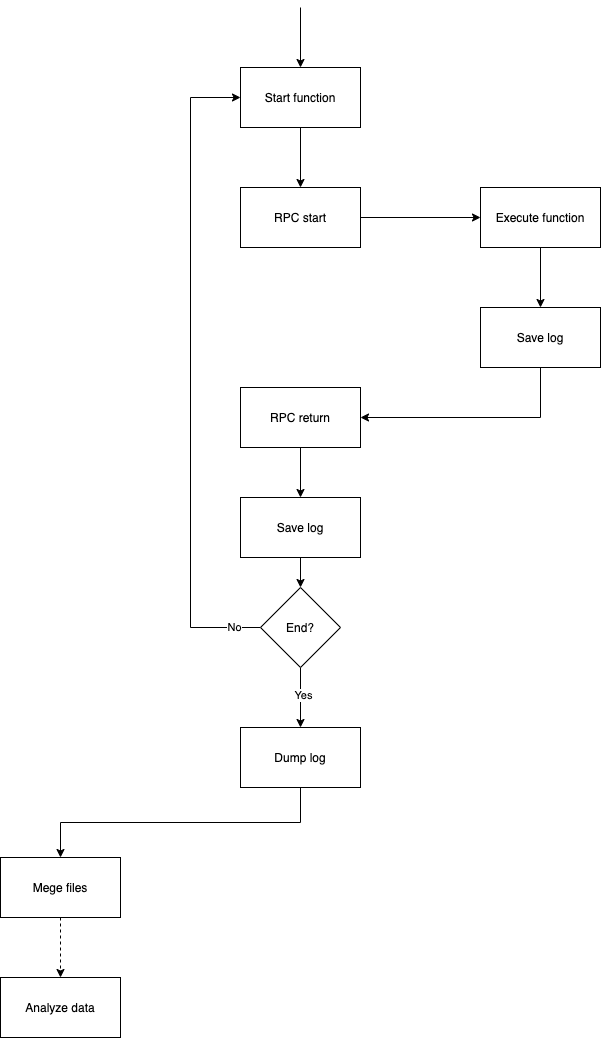
\includegraphics[width=0.6\textwidth]{schema.png}
        \caption{Jung's general functioning}
        \label{fig:schema}
    \end{figure}
    

    \section{Technologies and tools used}

        I used gRPC \cite{gRPCdocs} as the RPC library, since it seemed pretty straightforward and simple
        to use. There are plenty of examples in the documentation and a lot of languages are supported,
        including C++. On the other hand, Jung is independent from any library:
        its functions can be used directly from the code, even in a custom RPC implementation.\\

        The choice of language was pretty easy as well: Freud is built entirely in C/C++, so using the same
        language would increase compatibility. The only choice I had to make was regarding the version:
        I went with C++17 to benefit from the \texttt{filesystem::exists()} function, which I used to check
        for the existence of previous log files.\\

        To simplify development and testing, I also packaged an auto-building Docker image 
        (\url{https://hub.docker.com/repository/docker/steeven9/jung}) with the example server in it.
        This way I could keep the server running on another machine and, for example, test the network times
        from another remote location.


    \section{Issues}\label{sec:issues}

        The only major problem I had - which I believe to be very common - was that I made some
        design choices in order to initially simplify my job, but then, with the addition of
        new features or to fix certain problems, I had to change my approach. The direct consequence was that I
        had to rewrite some large parts of the code and data structures to adapt to the new requirements.\\
        
        One instance of the aforementioned problem is that I had to develop some particular encodings
        to represent the function parameters, since I had to convert from data (the running code) to text
        (the log file) and vice versa. More specifically, I chose to represent the values as 
        \texttt{name\=type\&value} (e.g. \texttt{asd\=int\&12} for an integer named \texttt{asd} of value 12);
        this added a supplementary layer of encoding/decoding when saving and reading the data to/from the
        text files.\\

        When we first started testing the integration with \texttt{freud-statistics}, since I was unable
        to see what was in the binary file, I had troubles checking if I was dumping the metrics correctly,
        resulting in some weird-looking statistics. With Daniele's help, we managed to make sense of
        the output and find the offending code parts to patch.\\

        And of course, I had my fair share of miscellaneous issues with pointers, segmentation faults and 
        general weird behaviors. As a positive note, in the process I somehow created a program that frees
        memory as you run it:

        \begin{figure}[H]
            \centering
            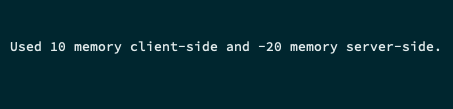
\includegraphics{memUsage.png}
            \caption{A very peculiar memory usage}
            \label{fig:memUsage}
        \end{figure}

        Another problem we ran into was that we were unable to get \texttt{freud-statistics} to find a
        regression, despite our data was clearly a good candidate for it. Turns out we simply didn't have a
        good enough p-value, which was easily fixed by getting more samples, as shown below.

        \begin{figure}[H]
            \centering
            \begin{subfigure}[b]{0.49\textwidth}
                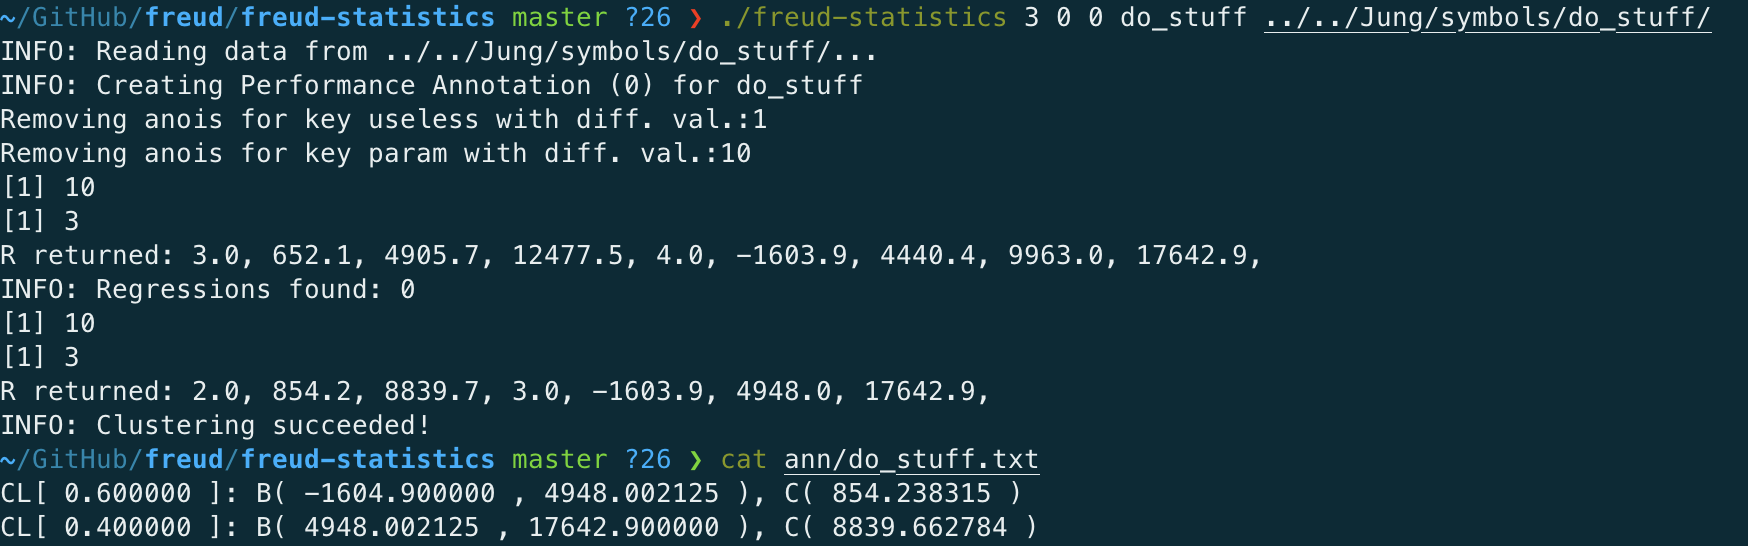
\includegraphics[width=\textwidth]{result.png}
                \caption{Not enough data points}
                \label{fig:result1}
            \end{subfigure}
            \hfill
            \begin{subfigure}[b]{0.49\textwidth}
                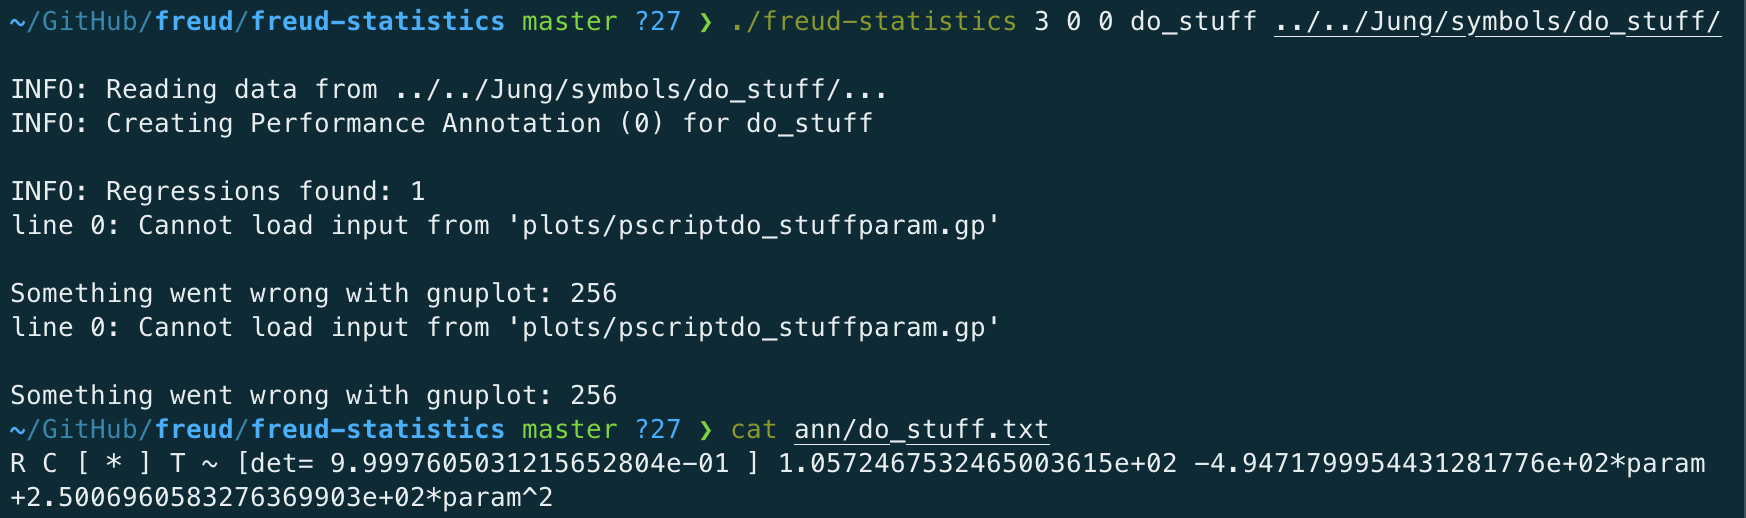
\includegraphics[width=\textwidth]{result_correct.png}
                \caption{With enough data points}
                \label{fig:result2}
            \end{subfigure}
            \caption{The results of our test program}
            \label{fig:fullresult}
        \end{figure}


\chapter{Evaluation}

    % Code validation, analysis of results and practical applications, personal experience (?)

    Referring to the task list in section \ref{sec:requirements}, I can assert that I successfully implemented
    all the required features. The results the library provides are accurate (to a certain extent) and I think
    that the code is pretty solid. Alas, time and coding constraints limited the amount of testing I could do,
    meaning that the performance analysis has been tested only with the demo program I made.


    \section{Testing}

        Due to the complexity and particular nature of the software, I decided to not implement any automated
        tests. Opposed to test-driven development, I had a more unstructured way of iterating over the code,
        since the functionality had to be checked by hand by comparing the produced log files with the program.
        Therefore, the effective coverage is 0\%, but as someone once said:\\

        \begin{quote} 
            \centering 
            \textit{"Tests don't prove correctness"}
        \end{quote}


    \section{Demo}

        In this section you can find instruction on how to run a demo program and analyze the obtained data.\\

        To install and compile all the required software, simply run the \texttt{install.sh} script from the Jung repository.
        In case of failure, please refer to the READMEs of each project for more information.\\

        First, start the server:\\

        \texttt{\$ ./jung\_server}\\
        
        While in another shell, run the client:\\
        
        \texttt{\$ ./jung\_client}\\

        \textit{Note: if you run the server on another machine, you can pass the \texttt{---target=HOSTNAME}
        % three dashes in the sentence above render correctly dunno why leave it like that
        argument to the client.}\\

        Then, with both the client and server log files in the root folder, merge the traces:\\

        \texttt{\$ ./trace\_merge}\\

        This will produce the binary data (under \texttt{symbols/}) and a summary of the execution
        (\texttt{trace\_log.txt}).
        We can then run Freud's analysis tool:\\

        \texttt{\$ cd ../freud/freud-statistics}\\

        \texttt{\$ ./freud\_statistics 3 0 0 do\_stuff ../../Jung/symbols/do\_stuff/}\\
        
        \textit{Note: this is an example, refer to Freud's documentation for details and usage.}\\

        This should find a nice regression and plot it. That's it!


\chapter{Conclusions}

    % Results wrt objectives, limitations

    I consider the results I obtained pretty satisfying: I managed to realize a working application
    that complies with the requirements and could be used in the field to measure actual systems
    (with some limitations, of course). The whole project was a great learning experience, both
    in terms of development and project management; in addition to refreshing my C++ skills, I
    experienced carrying out a large-ish project on my own, with deadlines and constraints.\\

    I would like to add that the way my advisor and I organized the work was very helpful: small
    steps and weekly meetings allowed to iterate quickly over the code and to keep 
    relatively on track with the schedule. As a matter of fact, the only discarded feature,
    testing on third-party applications, was not mandatory for the completion of the project.\\

    I'd like to thank Antonio, my advisor, for the opportunity and for guiding me throughout
    this project; Daniele, Freud's author, for his support and help
    understanding his software; my friends Sasha and Brites for their direct contribution;
    and last but not least everyone that supported me during these tiring times.


	\section{Future work and possible developments}

        While this project can be considered a success, there are still a number of improvements
        that could be implemented. For example a better handling of the data dumping via a separate thread:
        as of now every function writes the buffered metrics to the log file when it finishes executing. While this
        is barely noticeable on a small scale, it could add a significative overhead under large loads
        or in performance-critical systems.\\

        A crucial missing part is an actual instrumentation like Freud's, either with PIN or another
        library, allowing the user to work on the executables instead of changing the source code.\\

        Another possible improvement would be to support more complex features as parameters, like structs.
